% Chapter 2

\chapter{Hardware} % Main chapter title

\label{hardware} % For referencing the chapter elsewhere, use \ref{Chapter1} 

\lhead{Chapter 2. \emph{Hardware}} % This is for the header on each page - perhaps a shortened title

%----------------------------------------------------------------------------------------

\section{Inverter Systems Overview}

Power inverters are used for converting the DC power output of photovoltaic (PV) panels, batteries, or other DC sources into the AC power used in power grids worldwide. Our microinverter has three main power conversion stages, namely the DC/DC boost, H-bridge, and output filter. We will refer to the combination of H-Bridge and switching scheme frequently throughout this work simply as `the inverter.'  What we refer to as `the inverter' consists of an H-Bridge and transistor driver hardware that creates the pseudo-sinusoidal wave from the high voltage DC output of the boost. The inverter is of central concern in this work, and in particular, the pseudo-sinusoidal waveforms that result from our control scheme - these were mentioned briefly in Sections \ref{squareApproach}, \ref{pwmApproach}, and \ref{hybridApproach}, but will be discussed in detail in Chapter \ref{Chapter5}, Section \ref{fourier} - however, an inverter cannot operate in a vacuum. Therefore, we must first offer some background on the complete hardware system supporting the operation of the inverter system as a whole shown in Figure~\ref{solarBlock}. The following subsections will provide a detailed account of the role that each component part plays in the system.

\subsection{Logic Power Supply}

Logic power is sourced from the solar panel via a buck converter IC; a buck converter is an efficient means of converting high DC voltages into smaller DC voltages without generating an excess of waste heat, as is typical with LDO regulators. The buck converter steps input voltage down from approximately $35-45V$ to $12V$. To combat the relatively high harmonic content of the buck converter and the nefarious effect it would ave on our sensitive analog circuitry, we use LDO's to produce stable, and much cleaner, $5v$ and $3.3V$ rails for the supporting cast of hardware on our inverter - namely, the microcontroller, FET gate drivers, and op-amp sensing circuits. 

A logic power supply is required for the inverter board to run the microcontroller, driver circuits, and peripheral sensor network. Three different voltage rails were needed at $12V$, $5V$ and $3.3V$. The input from the solar panel was utilized to create these different power rails through a small connection circuit. Efficiency of this type of system is considered crucial, so cascaded switching DC/DC buck converters were used to create the $12V$ and $5V$ rails. A fast responding low-dropout linear regulator created the final $3.3V$ from the $5V$ rail. The circuit schematic for the logic power supply is shown in Figure~\ref{logic power fig}.

A variety of features were added to the front input interface for system protection and functionality. There are two options for sourcing power to the inverter board: banana jack connections for solar input and a DC barrel jack plug for testing input. These two circuits are configured so that only the barrel jack will source power if both happened connected and energized at the same time. Two switches are included for toggling the DC jack input and for switching conversion power into the main system. A ten amp blow fuse is included in series with the input to the inverter to prevent damaging short circuit conditions. A green LED on the $3.3V$ rail turns on to show the system is receiving power.
\subsection{Boost Converter}
The boost converter steps up the relatively low voltage sourced from one or two PV panels while implementing maximum power point tracking (MPPT) to keep the system operating near peak efficiency - this stage is critical for maximizing return on investment (ROI) in the face of the non-linear characteristics of the PV panel. The boost circuit trades current for voltage, much like a transformer, by harvesting the inductive kick of an inductor hooked up to a switch. By the fundamental relationship
\begin{equation}
V=L\frac{\delta i}{\delta t}
\end{equation}
 we see that the faster we can change current through the inductor, the larger voltage spike we can capture. This `capture' is done with a diode and capacitor circuit.

A generic boost converter circuit is shown in Figure~\ref{genericBoost}. The operation of a boost converter has two distinct phases depending on the switching mode of the power transistor. In this design, the gate of a MOSFET is sent different logic values at a specific duty cycles through PWM. When the drive circuit outputs logic high in Figure~\ref{genericBoost}, the drain to source path will conduct since the MOSFET is in the saturation region. This provides a path to ground for the current flowing through the inductor and reverse biases the clamp diode. While the transistor remains on, input current causes energy to be built up in the magnetic field of the inductor coil. Then logic low is sent to the MOSFET to shut it down. Considering the sudden change in current flow, a large voltage kickback occurs across the inductor and forward biases the diode. Current now can flow to charge the output capacitor and feed the load.

\begin{figure}
\centering
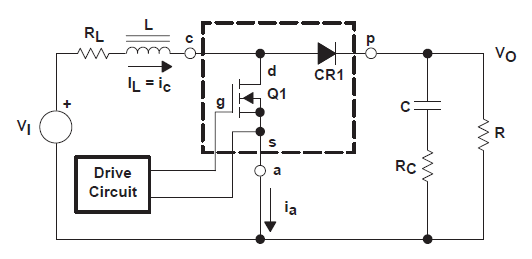
\includegraphics[width = 3.5in]{Generic_Boost_Converter.PNG}
\caption{Traditional Boost Converter Circuit}
\label{genericBoost}
\end{figure}

When the MOSFET is conducting, the output capacitor provides power to the load until it receives new charge during the second switching mode. A large ripple current flows through the inductor as the switching takes place. Boost converters can operate in two different ways depending on inductor current values. Continuous conduction mode (CCM) happens when the inductor current remains greater than zero at all times. CCM ensures that the voltage gain function remains a in linear relation solely with duty cycle $D$ as shown in Equation \ref{CCM Eq}. Discontinuous conduction mode (DCM) occurs when inductor current drops to zero during a switching cycle. The gain function for DCM, shown in Equation ~\ref{DCM Eq}, is more complex since it includes additional circuit parameters like inductance and is dependent on the load. 

\begin{equation}
\frac{V_{out}}{V_{in}} =  \frac{1}{1-D}
\label{CCM Eq}
\end{equation}   

\begin{equation}
\frac{V_{out}}{V_{in}} = 1 + \frac{V_{in}D^2T}{2LI_{out}}
\label{DCM Eq}
\end{equation}

The Sharp solar panels we are using feature a nonlinear output voltage and current relationship which depends on lighting conditions as shown in Figure~\ref{panelCharacteristics}. Maximum output power for the $170W$ panels occurs at $V_{pv,max}=34.8V$ and  $I_{pv,max} = 4.9A$. Boost output voltage is based on the minimum value needed for the $120V_{rms}/0.707 = 169.73V$ peak value required for the DC/AC inverter stage input. Maximum rated power of $200W$ is an upper limit selected for this design considering the solar panel approach with microinverter topology. Switching frequency is set at $50 kHz$ based on recommended ranges and to compare to the TI Solar Explorer Development Board also used in this project.\cite{SharpPanel}

\begin{figure}
\centering
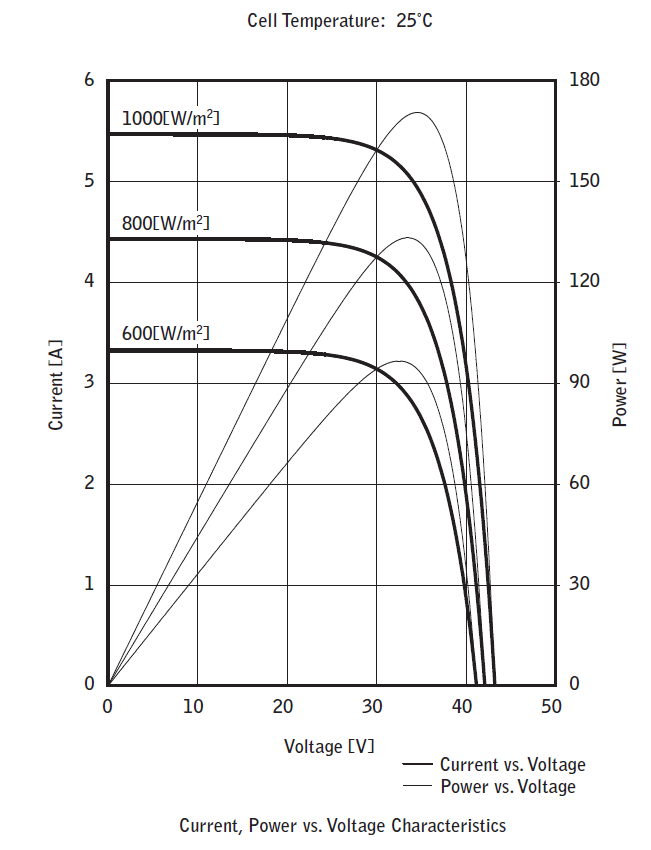
\includegraphics[width = 3.5in]{solar_v_vs_i.PNG}
\caption{Solar Panel IV Characteristics\cite{SharpPanel}}
\label{panelCharacteristics}
\end{figure}

The process of designing the boost circuit hardware involved a review of application notes and running PSPICE simulations. The voltage at maximum power of the PV panels $V_{pv,max}$ was selected for primary simulation testing. Calculations were performed to best select power components for operation of the boost converter at high power values. Component requirements for SMPS applications also influence the material composition options for parts. An example of this is the need to use electrolytic capacitors to obtain necessary voltage ratings and storage capabilities. The main design steps consider power dissipation, thermal limits, critical inductance, and critical capacitance. The PSPICE circuit encapsulating the entire boost converter design is shown in Figure~\ref{boostCrct}. The electrical specifications of this boost converter are listed in Table~\ref{specsBoost}.
\\ 
\begin{table}
\centering
\begin{tabular}{|c|c|}
\hline
 Parameter & Value \\
 \hline
 $ V_{in} = V_{panel}$ & 0V to 43.2V DC \\
 \hline
 $ I_{in}$ & 5.47A DC max \\
 \hline
 $ V_{out}=V_{load} $ & 200V DC max \\
 \hline
 $ I_{out} $ & 1.18A DC max \\
 \hline
 $ P_{rated} $ & 200W \\
 \hline
 $ f_{switching} $ & 50 kHz \\
 \hline
 $\bar{\eta} $ & 83.84 \% \\
 \hline
\end{tabular}
\caption{Electrical Specifications for Boost Converter}
\label{specsBoost}
\end{table}

\begin{figure}
\centering
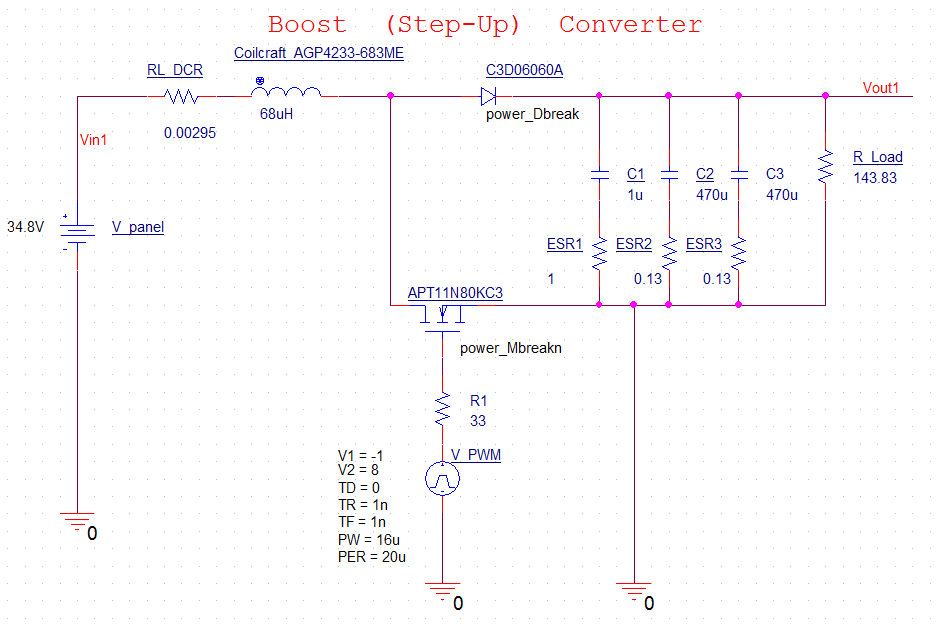
\includegraphics[width = 3.5in]{Boost_Circuit.PNG}
\caption{PSPICE Boost Converter Simulation}
\label{boostCrct}
\end{figure}

The operation of the boost converter in PSPICE required a switching signal to control the power MOSFET. Implementation of the converter will utilize function generator logic signals and Silicon Labs gate driver circuits for MOSFET switching. This simulation uses a variable duty cycle for continuous switching at the set frequency. This configuration is currently being run open-loop, but will include a compensation feedback control system to maintain stable output voltage in the final design. The solar panel $34.8V$ input at max power requires a duty cycle set at $80.13\%$ for the PWM switching signal to achieve $169.73V$ out. A load of $143.83\Omega$ is connected at the output to simulate max power current draw and realize the $200W$ capability of the system. Real output power will be less in practice due to additional inefficiencies, panel operating conditions, and sourcing configuration capabilities. The output voltage, current, and power of the boost converter, as it approaches steady-state conditions from start-up, are shown in the simulation results of Figure~\ref{boostApproachSteady}. 

\begin{figure}
\centering
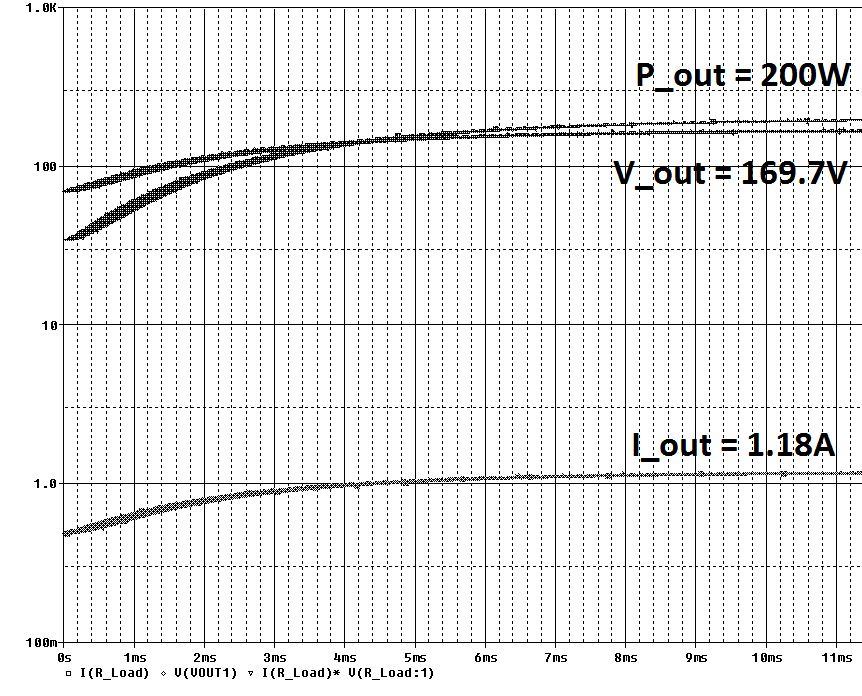
\includegraphics[width = 3.5in]{Boost_Power.png}
\caption{Boost Converter Approaching Steady State}
\label{boostApproachSteady}
\end{figure}

The simulation and prototype boost circuits have open-loop operation such that manual variation of duty cycle is required to obtain a certain output. Since the solar panel voltage can vary, the simulation circuit runs at a minimum of 20V to check that the needed output voltage can be maintained. The simulation results confirm this with $V_{out}=169.73V$, $V_{pv,in}=20V$, and a new duty cycle set at 89.25\%. 

This boost converter was designed to operate in continuous condition mode (CCM). This was achieved by selecting an inductor value above the calculated critical inductance and by making sure it has appropriate current handling capabilities. CCM requires the average inductor current to be larger than at least half of the load current. This is factored into the inductance calculation of Equation ~\ref{Lcrit Eq}.  Figure~\ref{inductorCurrent} shows the rippled inductor current during CCM and the MOSFET switching signal that creates these dynamic effects. 

\begin{equation}
 L_{critical} \ge \frac{R_{load,maxpower}D(1-D)^2}{2f_{sw}}= 50 \mu F
\label{Lcrit Eq}
\end{equation}

The series resistance of the inductor does not generate enough heat to justify heatsinking considering its large copper construction but it still dissipates power as estimated in the following equation.

\begin{equation}
P_L = (I_{in,rms})^2R_L = (5.47A)^2(0.025\Omega) = 0.75W 
\end{equation}

\begin{figure}
\centering
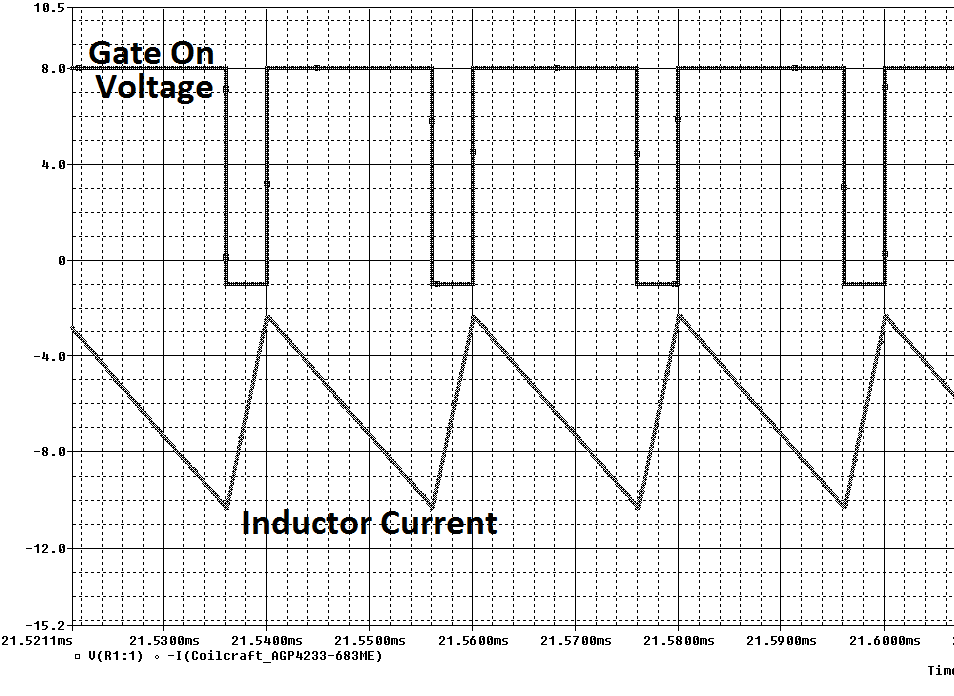
\includegraphics[width = 3.5in]{Boost_Inductor_Current_Steady_State.png}
\caption{Switching Signal and Inductor Current}
\label{inductorCurrent}
\end{figure}


The clamp diode was selected to be a Silicon Carbide (SiC) Schottky since it offers fast recovery times with low reverse recovery charge $Q_{rr}$ for reduced switching losses. Since the diode resides in the power conduction path, energy dissipation was analyzed. The diode was modeled as a series circuit of a temperature dependent voltage source $ V_{diode}$ and resistance $R_{diode}$.\cite{CREE}
\begin{equation}
 V_{diode} = \alpha T_{junction}+V_{diode,0} =  0.95V 
\end{equation}
\begin{equation}
 R_{diode} = \beta T_{junction}+R_{diode,0} = 0.103\Omega
\end{equation}
\begin{equation}
 P_{cond} = {I_{diode,rms}}^2R_{diode}+I_{out,max}V_{diode} = 2.76W
\end{equation}
\begin{equation}
 I_{diode,rms} = \frac{I_{out}}{\eta} \sqrt[]{ \frac{16V_{out}}{3 \pi V_{in}}}= 3.99A
\end{equation}
\begin{equation}
P_{switching} = Q_{c,diode}V_{out}f_{sw}=0.14W
\end{equation}
\begin{equation}
 P_{dissipation,diode,total}= P_{conduction}+P_{switching}=2.91W 
\end{equation}
The $2.91W$ that the diode dissipates is significantly lower than the $136.3W$ rating for the device. Regardless, heat sinking it with a TO-220 bolt-on type sink is still a good practice.

The power MOSFET selected for the boost converter has very adequate voltage and current handling capabilities for the $200W$ design. The transistor experiences both switching and conduction power consumption which are shown in the following equations along with a thermal analysis for heatsinking.

\begin{equation}
V_{off} = V_{out} + V_{f,diode} = 171.53V
\end{equation} 
\begin{equation}
P_{cond} = \frac{1}{2}V_{off}I_Df_{sw}(t_{rise}+t_{fall}) = 0.68W
\end{equation}
\begin{equation}
P_{sw} = C_{oss,FET}{V^2}_{off}f_{sw} = 1.11W
\end{equation}
\begin{equation}
P_{dissipation} = P_{cond} + P_{sw} = 1.79W
\end{equation}
\begin{equation}
P_{limit} \leq \frac{T_J-T_A}{R_{\theta JA,max}} = 2.02W > 1.79W
\end{equation}
\begin{equation}
R_{\theta JA,new} = \frac{T_J-T_A}{P_{diss}} = 71.02\frac{\,^{\circ}\mathrm{C}}{W}
\end{equation}
\begin{equation}
R_{\theta SA} \leq R_{\theta JA,new} - R_{\theta JC} - R_{\theta CS} = 63.73\frac{\,^{\circ}\mathrm{C}}{W}
\label{FETsink}
\end{equation}

The $2.02W $ and $ 1.79W$ power losses calculated are close and thus heatsinking is required. The standard TO-220 heatsink with a thermal resistance of $25\frac{\,^{\circ}\mathrm{C}}{W}$ meets the criteria calculated in Equation ~\ref{FETsink}.

The output capacitance was designed as a parallel arrangement of two values of capacitance for fast and slow transient response. This increases the total capacitance while reducing the equivalent series resistance (ESR) of the combination. This helps reduce the output voltage ripple of the boost converter. Since DC voltage output is required, a maximum ripple of 50mV = $\delta V_{out}$ is selected as the tolerance. To achieve this voltage ripple design, a critical minimum output capacitance was calculated.\cite{hasaneen}
\begin{equation}
D = 1 - \frac{V_{out}}{V_{in}} = 79.81\% 
\end{equation}
\begin{equation}
C_{critical} \ge \frac{V_{out}D}{F_{sw}\delta V_{out}R_{load,maxpower}} = 370 \mu F
\end{equation}

Voltage and current ratings for components are determined through worst case calculations.\cite{kwasinski} 
\begin{equation}
I_L = I_{diode} = I_{drain} = \frac{2}{\sqrt[]{3}}I_{in,rms} 
\end{equation}
\begin{equation}
 V_{cap} = V_{out} = 1.5V_{out,typ} = 2(169.73V) = 254.6V 
\end{equation}
\begin{equation}
 V_{diode} = V_{DS,FET} = 1.5(169.73V) =339.46V  
\end{equation}
\begin{equation}
I_{cap} = I_{out,rms} = 1.18A 
\end{equation}

Figure~\ref{boostCompleteSchematic} contains the complete boost schematic which has many design concepts inspired by the Texas Instruments Solar Explorer Development environment.\cite{tiAppReportControl} The circuit schematic shows the conventional boost converter, the associated sensing and signal conditions circuits, and the gate driver circuit. The energy conversion portion of the boost board is shown in Figure~\ref{boostConverterCircuit} with an additional input filter capacitor bank. The sensing of PV panel voltage and output voltage consisted of basic divider circuits with MCU pin protection diodes as shown in Figure~\ref{VpvSenseCircuit} and Figure~\ref{VboostSenseCircuit}. The input PV current is measured with a shunt resistor IC with high common-mode rejection in Figure~\ref{IpvSenseCircuit}. The switching transistor current is measured with a differential op-amp configuration as shown in Figure~\ref{IswSenseCircuit}. Lastly, the switched MOSFET has a low-side gate driver IC taking in PWM as depicted in Figure~\ref{gateDriverCircuit}. 

The top layer of the PCB design is shown in Figure~\ref{boostPCBTop} and the bottom layer is shown in Figure~\ref{boostPCBBottom}. The first generation prototype boost board PCB was created using a LPKF Protomat M60 router. This machine allows modified PCB gerber files to be milled into two-layer boards from standard copper clad plates. The resulting unpopulated boost board is shown in Figure~\ref{unpopulatedBoostPCB}. The board was then populated with components into a completed circuit as shown in Figure~\ref{Built Boost} Testing of the boost circuit demonstrated its voltage gain capabilities with outputs reaching in excess of 120V during open-loop operation.

\begin{figure}
\centering
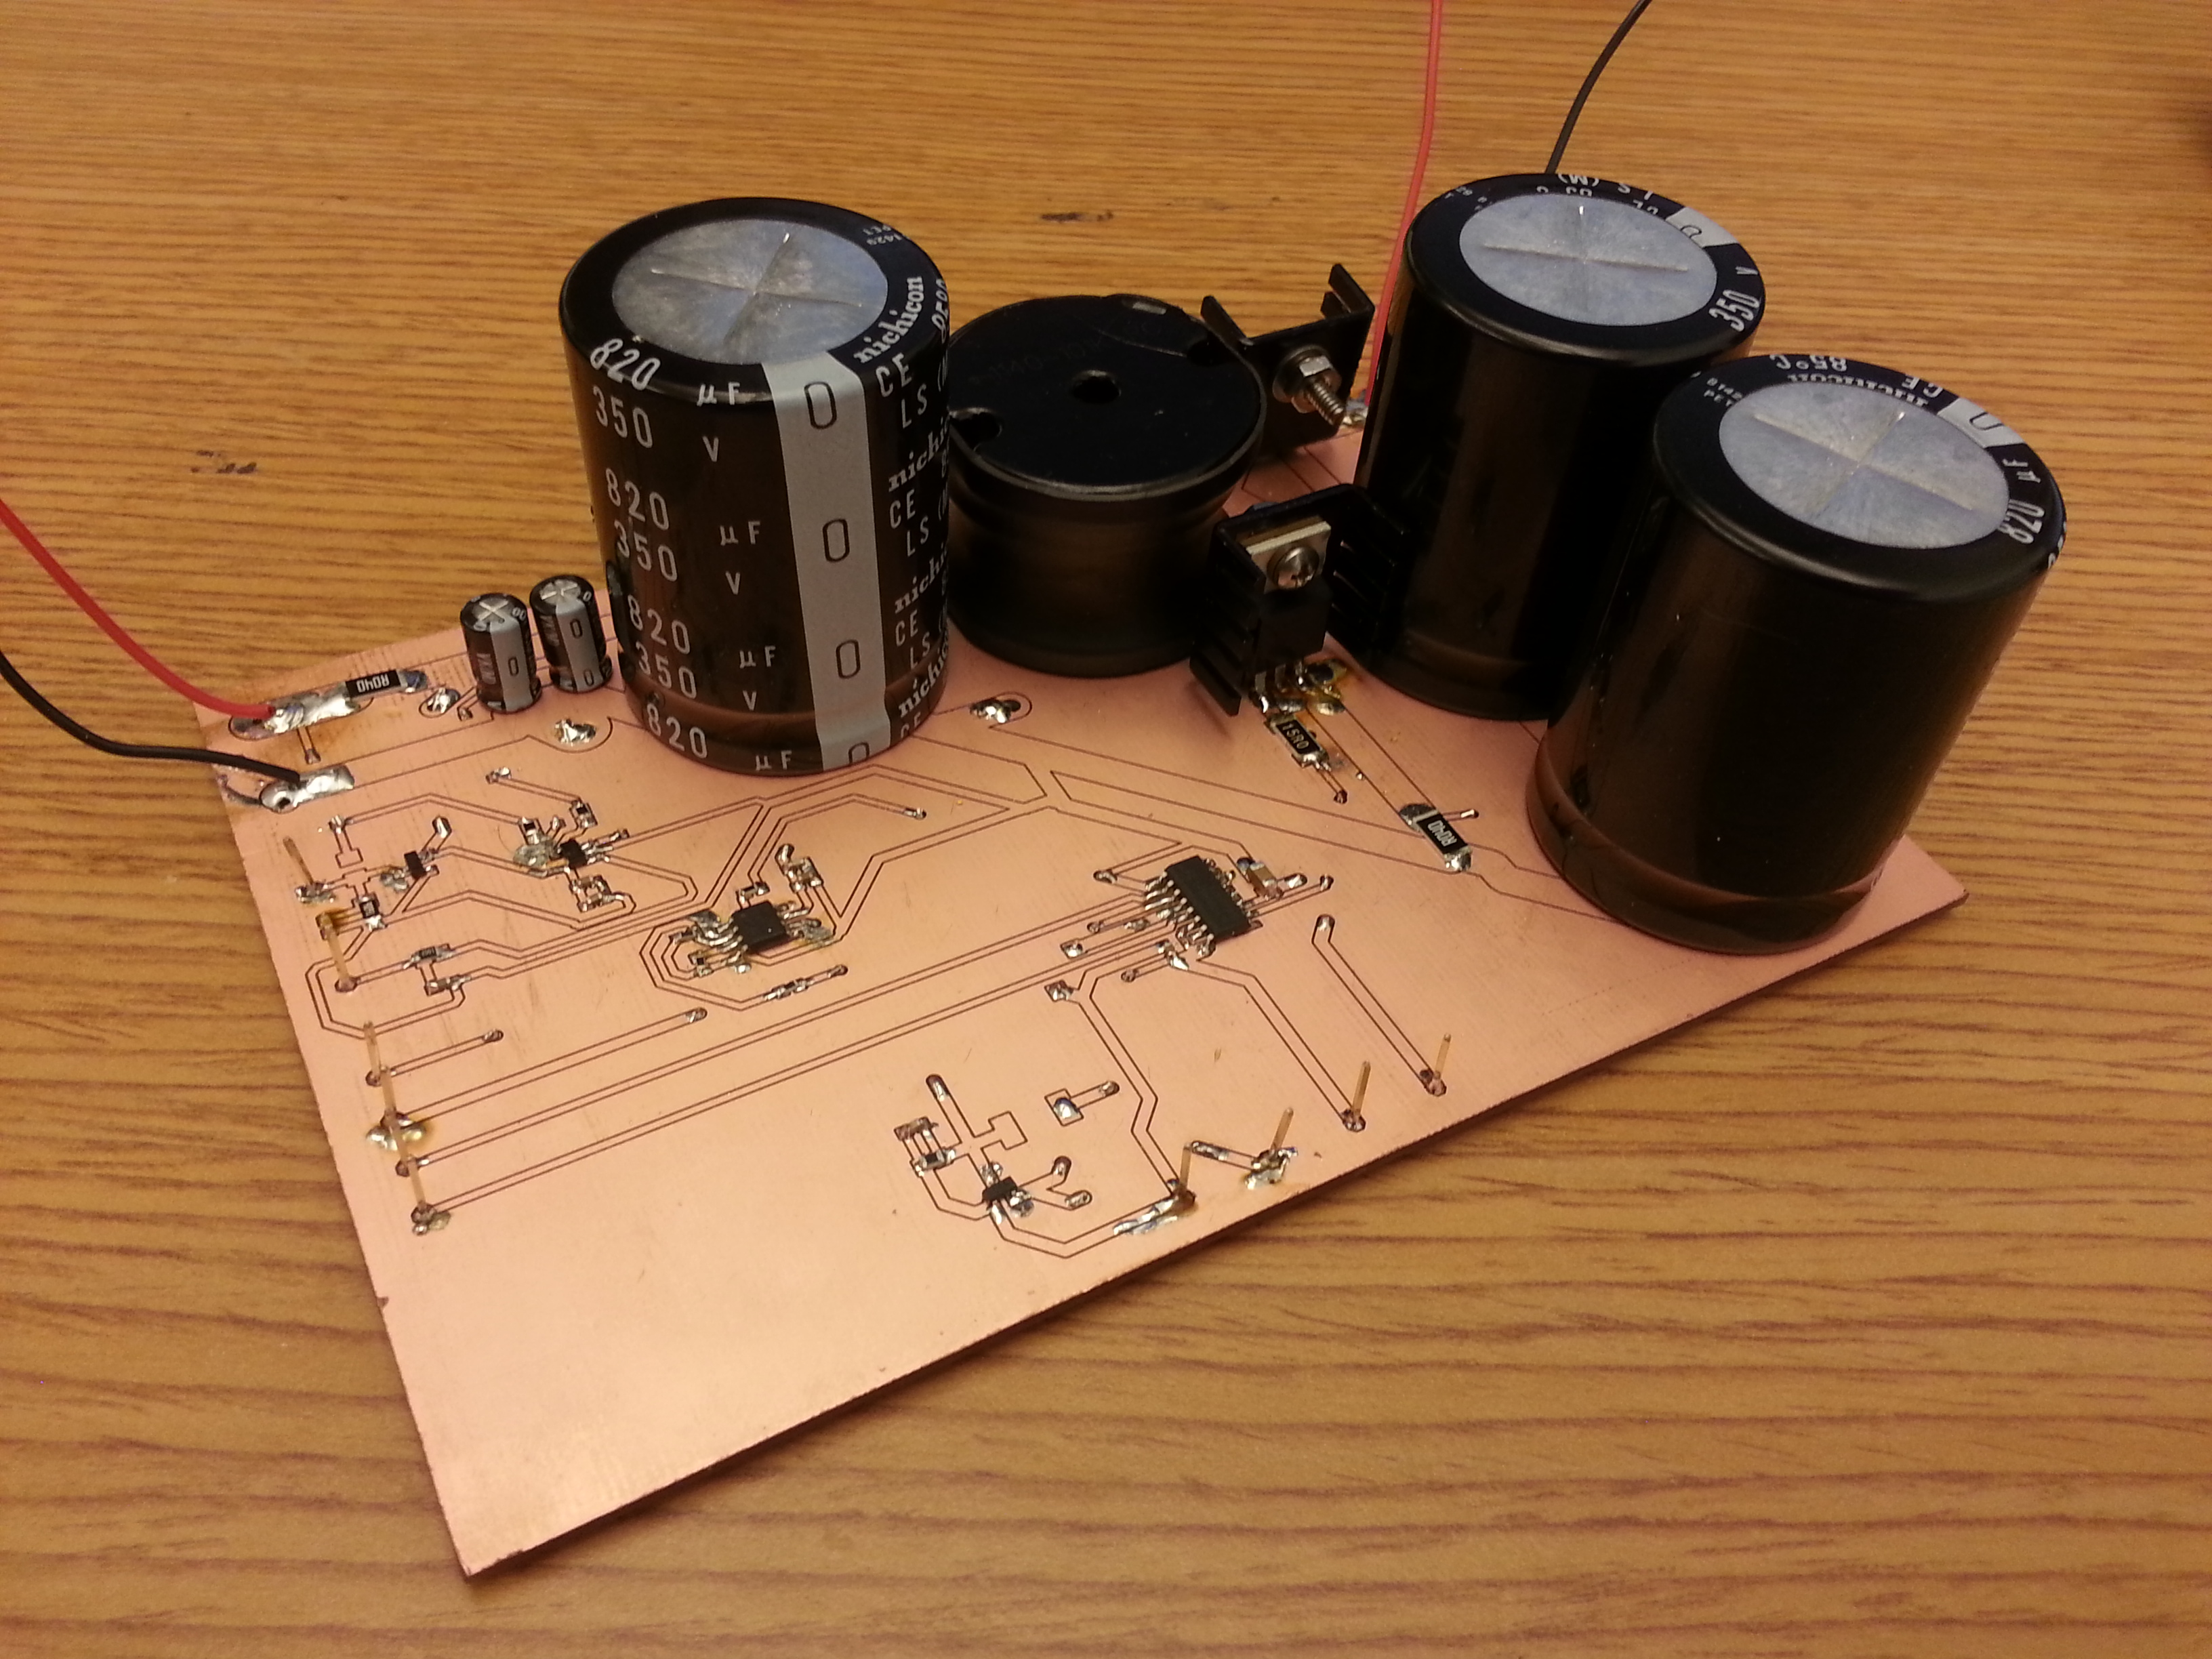
\includegraphics[width = 3.5in]{built_boost.jpg}
\caption{Assembled Boost Circuit}
\label{Built Boost}
\end{figure}

\subsubsection{Boost Converter Efficiency}
Energy conversion efficiency is an important factor for determining the effectiveness of the boost converter. Ideally, the circuit will have a 100\% power conversion rate but in practice this is not feasible. Losses occur during periods of conduction and switching due to parasitic resistances and capacitances.  Rates in the high ninetieth percentile have been achieved in some switching DC/DC converters but efficiencies falling more in the range of 90\% to 70\% are more common and can be deemed acceptable depending on the application. A first order estimate of the boost's efficiency $\eta_{est}$, with the MOSFET, diode and inductor loss considerations, is calculated in the following the following equation.

\begin{equation}
\eta_{est} = \frac{P_{in} - {(P_{sw}+P_L+P_D)}}{P_{in}} = 97\%
\end{equation}


This is an optimistic conversion efficiency and does not fully encapsulate an array of other possible factors such as component tolerances and capacitive equivalent series resistances. A deviation of 10\% is a fair engineering estimate on how much $\eta_{est}$ could drift. The boost converter circuit prototype allows efficiency testing under the constraints of a laboratory environment. Experimental efficiency $\eta_{exp}$ is calculated with the relationship shown in the following equation. The operating parameters of the test are: $V_{in} = 12V$,~ $R_{load} = 477.66\Omega$ , $F_{switching} = 50 kHz$. 

\begin{equation}
\eta_{exp} = \frac{P_{out}}{P_{in}} = \frac{{V_{out}}^2/{R_{load}}}{{V_{in}}{I_{in}}}
\end{equation}

The test uses different PWM duty cycles between 20\% and 73\% to obtain peak and average efficiencies as shown in the following equation.

\begin{equation}
\eta_{exp,peak} = 85.4\%, ~ \bar{\eta}_{exp} = 83.84\% 
\end{equation}


As the testing indicates with $\bar{\eta}_{exp}$, the boost converter operates well within the range of standard energy conversion efficiencies. The boosted output voltage compared to input voltage over different duties is shown in Figure ~\ref{Boost Converter Output Voltage Vs. Duty Cycle} and the voltage gain versus duty is shown in Figure ~\ref{Boost Converter Gain Vs. Duty Cycle}. These results demonstrate how increasing the duty closer to 100\% will increase the output voltage.

\begin{figure}
\centering
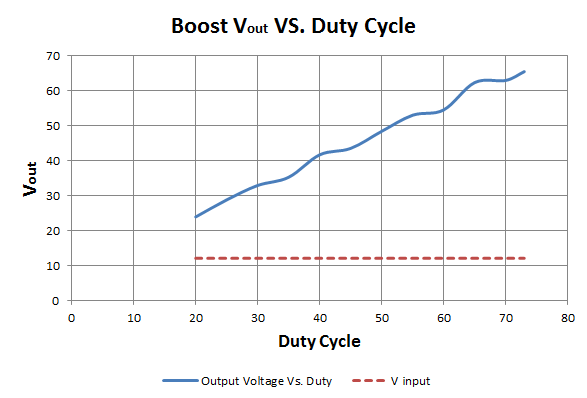
\includegraphics[width = 3.5in]{boost_out_vs_in.PNG}
\caption{Boost Converter Output Voltage Vs. Duty Cycle}
\label{Boost Converter Output Voltage Vs. Duty Cycle}
\end{figure}

\begin{figure}
\centering
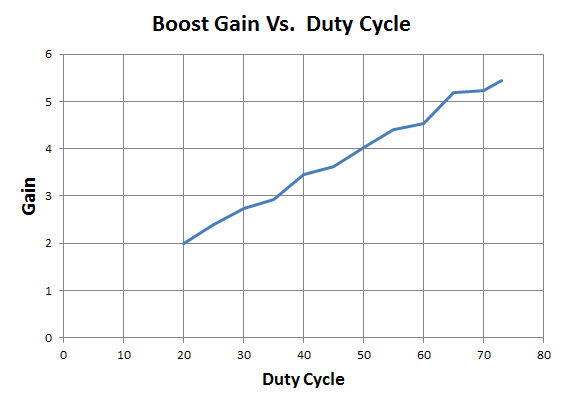
\includegraphics[width = 3.5in]{boost_gain_vs_d.PNG}
\caption{Boost Converter Gain Vs. Duty Cycle}
\label{Boost Converter Gain Vs. Duty Cycle}
\end{figure}



\subsection{H-Bridge}
Arguably, the lynch-pin of any inverter is the H-Bridge circuit. In order to generate a pseudo-sinusoid from a DC source, we must first have the means to switch this DC voltage on and off, and also to drive current bidirectionally. Thus, careful design of the H-Bridge circuit was a critical step in our development.

For a successful H-Bridge design, we needed to consider a number of factors including the speed of switching, deadband, transistor type, transistor gate drivers, thermal analysis, and careful layout due to the speed of the signals involved and the resultant EMI.

After some analysis of the algorithm, further discussed in Chapters \ref{Chapter3}, and \ref{Chapter5}, we found that the speed of switching with the hybrid algorithm - unlike the switching speed of PWM algorithms which modulate over a fixed carrier frequency - was highly dependent on the width of the tracking band. Consequently, there is also a dependence on the resolution of the ADC, and the frequency at which our interrupt is serviced. Through simulations in Matlab we were able to determine that the speed at which the algorithm caused the inverter to switch were well under 100kHz for a 'small-enough' tracking band. 

Because the switching speed is a function of width of the tracking band, sampling rate, and ADC resolution it is by no means a straightforward calculation to determine the frequency of switching. Contrast this to the PWM approach where this determination is trivial. In any case, because the switching speed was tunable by way of modifications to the with of the tracking band, it was decided that it was not necessary to go with more advanced FET technologies like Galium Nitride that are more than capable of switching in the MHz range under full load. 

Shoot-through is another important consideration with the H-Bridge circuit, as the possibility of a nearly direct path from power to ground can exist as the circuit switches from outputting +Vdc to -Vdc. To prevent this, a mandatory off time is implemented in software along with  hardware protection afforded us by the gate drivers. In the configuration of the PWM driver in our micro controller code, a 330ns deadband was implemented, based off of the 60MHz clock on the Piccolo. The drivers offer a nominal 70nS dead-time giving us robust, multi-tiered protection against shoot-through. 

For the transistors in the H-Bridge, we decided on field effect transistors, (FETs), and in particular the CoolMOS\textsuperscript{TM}
variety built by Infineon. The IPP60 comes in a standard TO-220 package allowing for the use of standard heatsinks, has a Vds max of 650V - about three times what we would need - and a maximum continuous current of 31 Amps. Additionally, these FETs have a very low gate charge (low capacitance, smaller switching losses), low Rds on, and great slew rate. The fact that the drain to source resistance is low helps with our thermal budget, and also means higher efficiency overall. Because of the bipolar switching that the hybrid algorithm called for, we felt that it was wise to over specify our switches. Finally, the freewheeling diode found on many H-Bridge circuits was not needed here since the diode inherent to the construction of the FET was sufficient to handle any expected back currents in our load. 

\subsubsection{Switching Loss and Conduction Loss}
One of the primary factors in the overall efficiency of a modern switching power supply is the switching loss inherent to FET technology, and also the conduction loss associated with $R_{DS}$ on, the resistance of the FET from drain to source while it is conducting. Switching loss occurs whenever the FET changes state, and can be roughly understood as the net amount of charge it takes to drive the gate of the device. This amount of charge corresponds to a loss of current that could have gone to drive the load in question. This effect can be mitigated in some cases with parallel capacitance at the gate, using `faster' FETs (higher slew-rate), and judiciously selecting the freewheeling diode\cite{switchingLoss}. Unavoidably, however, there is a trade-off between swithcing loss related to fast control signals of the H-bridge, or switching more slowly and dealing with bulky analog components and the loss associated with them. 

The heat sinks in our design are connected to the AC ground. Both the low-side and high-side transistors are insulated from the heat sink with thermal pads and insulating shoulder washers. According to the Transform application note we used as reference during our design, "For the high-side transistor, capacitance between the TO220 tab and the heat sink will add to switching loss, and so a thick and/or low permittivity insulator should be used."\cite{transphorm}

We chose the SI823x family of gate drivers from Silicon Labs, which have a built-in under voltage protection to prevent `nuisance trips' and to add noise margin to our control signal. The gate drivers utilize a bootstrap circuit to operate as both a high-side and low-side driver - this is to say that we can use N-type FETs for all four switching transistors. 

Because of the relatively high speeds involved with the H-Bridge, careful layout was especially important here. Parasitic capacitance on gate and drain loops are a main cause of overshoot and ringing in the circuit, and thus the total enclosed area between the gate drive and the FETs was kept to the absolute minimum. In order to minimize inductance in the output current path, high current power and ground planes were utilized. Small ferrite beads were used between the gate drive output and the gates of the FETs to reduce ringing cause by coupling of the drain current to the gate drive loop- these were found to be more useful than small resistances which are sometimes used \cite{transphorm}. High voltage SMD ceramic bypass capacitors were placed directly underneath either side of the H-Bridge circuit to minimize the series inductance in the circuit. 
  
\subsection{RLC Output Filter}
The output filter must attenuate high frequency switching noise while passing the 60Hz fundamental intended for standard loads. In a typical PWM design, the driver factor behind the cutoff frequency of the output filter is the carrier frequency of the PWM signal. In most cases, this carrier frequency is invariant, and therefore allows for a relatively straightforward design parameter during the time where components are selected. Of course, THD is also a primary driver of part selection and valuation of the analog components.

In order to ensure that the vector fields on the power plane are such that the hybrid algorithm can ensure forward invariance, and that the solution of the system converges to the tracking band in finite time, it is necessary that our design adhere to a set of constraints on the RLC filter described in \cite{ricardo}. 

Namely, our filter components must meet the following constraints: first, we must satisfy the condition that $LC\omega^2>1$ - this property ensures our vector fields are oriented correctly throughout the desired trajectory on the VI plane. Second, we have that the capacitor value must be determined by the output voltage amplitude and current amplitude by the relation:$\frac{I_l\omega}{V_c}$ where $I_l$ is the target output current, and $V_c$ is the target output voltage. From this final condition we observe that the value of the capacitance can be driven up by increasing the target current, decreasing the target voltage, or increasing the frequency of operation. 

Let's examine this mathematical condition through the lens of circuit analysis. By inspection, we note the similarity of this condition to the condition for resonance in a series RLC circuit - which is the subject of study in \cite{ricardo}. This condition is given by $\omega_0 = \frac{1}{\sqrt{LC}}$ Taking the square of both sides in the expression, find that $\omega_0^2LC=1$, and we see that the condition on the filter components given states that the resonant frequency of the circuit ought to be greater than unity. If we suppress the variable for capacitance in 
$LC\omega^2>1$ given the condition $C=\frac{I_l\omega}{V_c}$, we obtain:
\begin{equation}
\label{constraint}
L > \frac{V_c}{I_l\omega^2}
\end{equation}

The expression obtained in \ref{constraint} adds a considerable degree of inductance compared to that in a typical PWM inverter. It was considered initially that the quality factor, $Q$ might be at work in the conditions on the filter, but we find that the quality factor for the series RLC filter is given as $Q = \frac{1}{R}\sqrt{\frac{1}{LC}}$, and the analysis in \cite{ricardo} makes no mention of the damping term $R$. 

Subsequent testing on filters that do not adhere to this constraint must be conducted to determine the viability of this algorithm in applications in inverters in the sub-1kW range. Although we have not conducted research on filters for higher power systems, in the regions of interest for this paper this filtering constraint has proved to be quite costly and bulky. 

We constructed our filters using `power reactor' inductors from Triad magnetics. They are values at 35mH each if their coils are wires in series, or around 6mH if their coils are wound in parallel. To be clear, each inductor is constructed of a pair of inductors. Correspondingly, our maximum current decreases at the higher inductance, roughly $5A$ when wired in series, and maintains the rated inductance in the parallel configuration with a $10A$ rating. Inductors beyond this current rating were typically found to have lower inductances and prohibitvely high prices for our research. This limit on inductance is very much a materials science problem; as the current through the inductors increases, the cores used in their construction saturate and limit the effective inductance. 

Using the constraint given above, we sized electrolytic capacitors for our series RLC filter. Because electrolytics are polar devices, we needed to use a special confguration where we used electrolytic pairs to construct non-polar electrolytic capacitors. This was found to be a relatively common trick, but we performed several stress tests to verify the robustness of this solution. Regardless, electrolytics are understood to be the weak-link in the lifespan of inverters with their short mean time to failure at moderate to high temperatures. The final constructed filter on turret board is shown in Figure ~\ref{filterTurret}.  

\begin{figure}[h]
\centering
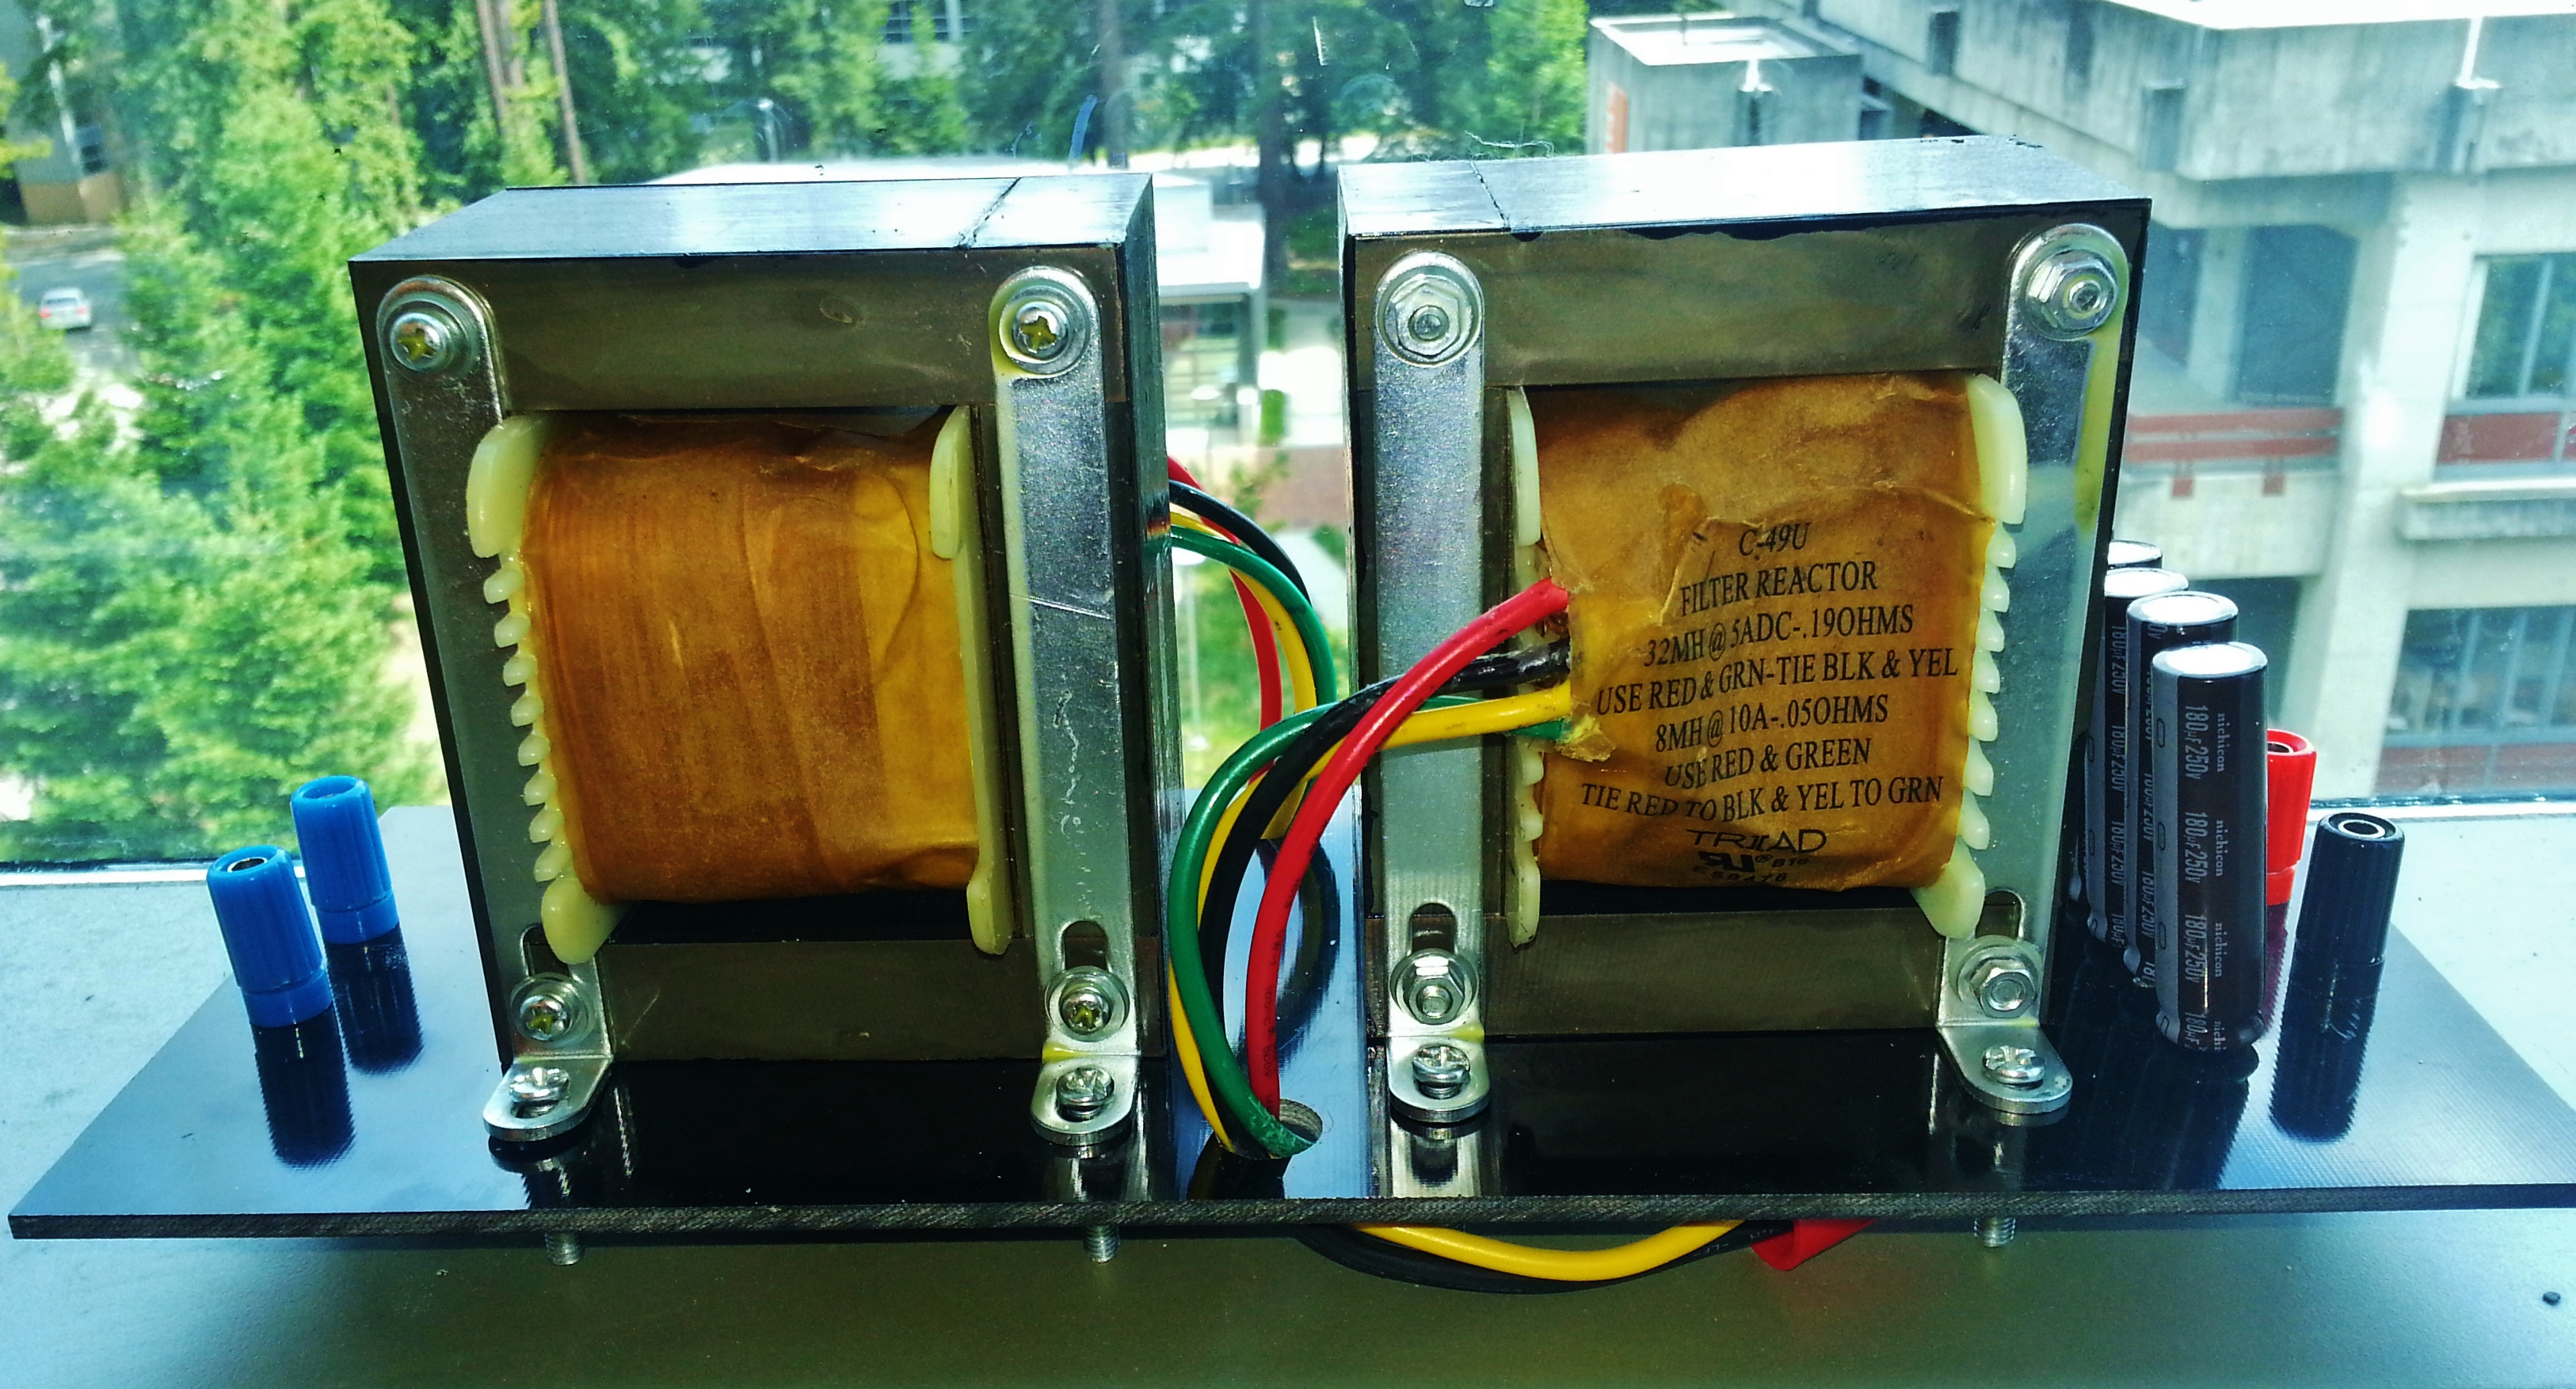
\includegraphics[width=3.5in]{filterTurret}
\caption{RLC Resonant Filter}
\label{filterTurret}
\end{figure}

\subsection{Feedback Sense}
The sensor network is important for the operation of the inverter since it allows the microcontroller to monitor voltages and currents for feedback control. Voltage dividers are used to measure high potentials around the boost converter and filter outputs. The inverter's AC output voltage is measured by a differential op-amp with a DC offset of $1.65V$ to allow for the input signal's negative potential swings. A differential comparator IC implements zero cross detection as the biased AC wave oscillates above and below the DC reference. 

Inverter output current is measured through the use of two shunt resistors in the low-side legs of the H-bridge. The small voltage drops on these $0.04\Omega$ resistors are conditioned by two differential amplifiers. The difference between the two signals from the legs is calculated by the microcontroller to evaluate the output current. A secondary Hall effect IC is inline with one of the H-bridge outputs so that it can noninvasively measure a signal linearly proportional to the AC current by using it's changing magnetic field.

\subsection{The Microcontroller}
At the core of our inverter system is the Texas Instruments F28035 `Piccolo' microcontroller. This embedded controller's internal architecture is optimized for the real time control of devices like switching power converters. The Piccolo has a control law co-processor that can operate complex feedback loops without burdening the main processor, freeing the central unit to perform higher level tasks. The device also features versatile pulse width modulation units which are connected to the general purpose outputs for driving the switching power transistors of the boost converter and H-bridge. 

With the myriad of choices available to designers of power systems, the task of selecting a microcontroller for a power conversion system is no easy task. The first step was to survey the current landscape and find some examples of the most popular microcontroller choices currently being used in power applications today. The controllers that we found most frequently were the dsPic family by Microchip, and the Piccolo family by Texas Instruments. The reasons that these two families have found dominance in this field became obvious: they were low cost, had detailed documentation and application notes for power conversion, and support for the 'real-time' control loops that our application demands.

With the choice narrowed down to two families of processors, the task of selecting a processor boiled down to a cost/benefit analysis between the two. Both had similar power consumption, but the TI family of Piccolo controllers came with the option of faster clock speeds, and correspondingly, faster ADC sampling times. Additionally, the resolution of the PWM and ADC modules was more precise than those of comparable Microchip controllers. The final check-box in the TI column was the tight integration of the Piccolo family of controllers with two of the power development boards that we were considering - the Solar Explorer by TI, and a competing offering by Transphorm. 

With code portability from our development kit to a final implementation being of paramount importance, it was decided that we should go with the Piccolo family. In particular, we chose the F28035 for its mix of speed, low-cost, and wide array of digital control capabilities including a unique co-processor feature known as the CLA which enables offloading of many control implementable in assembly. With the integration of this Control Law Accelerator or CLA, we are able to significantly increase the complexity of our algorithms for a given clock speed, while also running multiple state machines and servicing interrupts occuring at multiple frequencies - all while doing it \emph{faster} than would be possible on competing microcontrollers.

Our final hardware design includes anti-aliasing filters for all ADC inputs, and is capable of outputting the values measured at the ADC to DAC pins for debugging purposes. The system uses a 20MHz crystal to set the pace for a phase-locked system clock of 60MHz. External hardware in support of the microcontroller includes voltage protection diodes on GPIO and ADC pins, and isolated communication circuits allowing for the use of USB debugging while protecting against ground loops.

\subsubsection{USB-JTAG interface}
The Piccolo microcontroller supports JTAG boundary scanning for device programming and real time debugging. To connect through the JTAG circuit, several integrated circuit solutions are implemented on our inverter. Programming, or 
`flashing' the micro with code compiled on a workstation necessitates a USB connection to the inverter board. A Future Technology Devices International (FTDI) FT2232D is used to interface a mini USB with the micro by converting the signals to UART. This device also allows the configuration of an EEPROM flash memory array for use with the proprietary Texas Instruments XDS100 debugger use by the Code COmposer Studio IDE. The USB connection provides its own power to the JTAG conversion circuit, so galvanic isolation is used between the USB power supply and that of the main inverter board to prevent ground loops. Digital signals are sent between the two subsystems through a series of digital isolator ICs which use capacitive coupling. A Texas Instruments IC MAX3221 is present as an RS-232 driver/receiver for the serial RX and TX connections between the FTDI chip and the microcontroller.

\section{Photovoltaics}
Photovoltaics, more commonly known as solar panels or solar cells, operate by the principle known as the photoelectric effect. The description of this phenomena won Albert Einstein the Nobel prize in 1905. In this work, he described the quantized energy carried by photons. This energy was found to be $E=hv$, where $h$ is Plancks constant. If we have a pn junction with a thin, heavily doped $n$ region, then a depletion region exists between the two materials. This region is observed to extend primarily into the $p$ region with an electric field $E_0$. While we need electrodes to construct a `bulk' solar cell, these electrodes must also allow light to enter the device. This is typically done by forming electrodes into thin finger like structures on the surface. Additionally, antireflective coatings are typically applied to maximize light incident upon the device \cite{materials}.

If we engineer a semiconducting material with a bandgap tuned to the wavelengths of photons emitted from the sun, then the photons strongly interact with the material and are absorbed. The net effect is the emission of electrons which result in an open circuit voltage between the $p$ type and $n$ type materials. If we complete this circuit, we will obviously obtain an electric current which can be used to drive DC loads - this current is known as a photocurrent. 

The engineering of semiconducting materials that can interact with broad ranges of wavelengths is the subject of much research, but is entirely beyond the scope of this report. Rather, we are more concerned with harnessing the direct photocurrents from PV systems readily available today and turning them into alternating currents. 

In order to achieve this goal we must understand the non-linear relationship between the power generated by solar panels and their operating conditions. From an electrical standpoint, a solar cell is best represented through an engineering circuit model of a current source in parallel with a diode. Two significant parasitic resistances are included in series and parallel positions in the model to account for the physical factors of a solar cell. The current source is responsible for the photocurrent $I_{photo}$ generation due to incident light and will feed DC loads present on the cell's terminals. The diode contributes to a dark current $I_{dark}$ which counters the positive photocurrent and accounts for cell loading. The circuit model of an individual solar cell is shown in Figure ~\ref{circuitModel}. \cite{soteris}

\begin{figure}
\centering
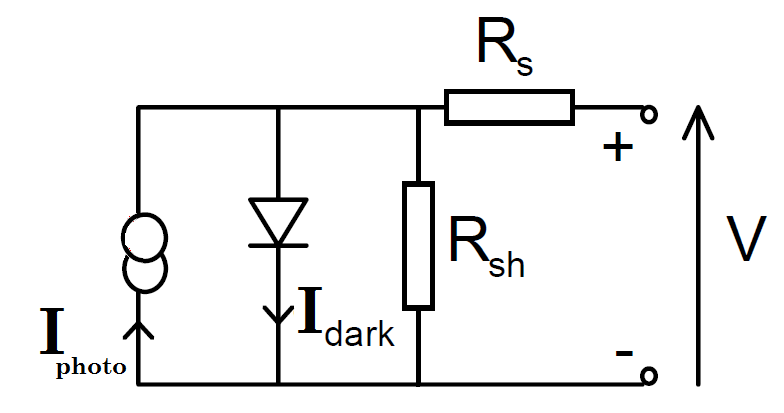
\includegraphics[width = 3.5in]{solar_cell_model.PNG}
\caption{Circuit Model of Solar Cell}
\label{circuitModel}
\end{figure}

Depending on the load, two important parameters can be determined for a solar cell: open circuit voltage $V_{oc}$ and short circuit current $I_{sc}$. The short circuit current will be directly proportional to the intensity of a certain light frequency spectrum for the solar cell and $I_{sc}$ will have a finite maximum value based on the efficiency of the panel. The open circuit voltage occurs when there is no load, massive impedance on the cell terminals, and the dark current through the shunt diode derails any photocurrent. The diode potential drop creates the largest effects on the voltage profile of the solar cell and adds to the non-linearity of the I-V plot for the system as shown in Figure ~\ref{Output Voltage Vs. Current of a Solar Cell}. \cite{soteris}

\begin{figure}
\centering
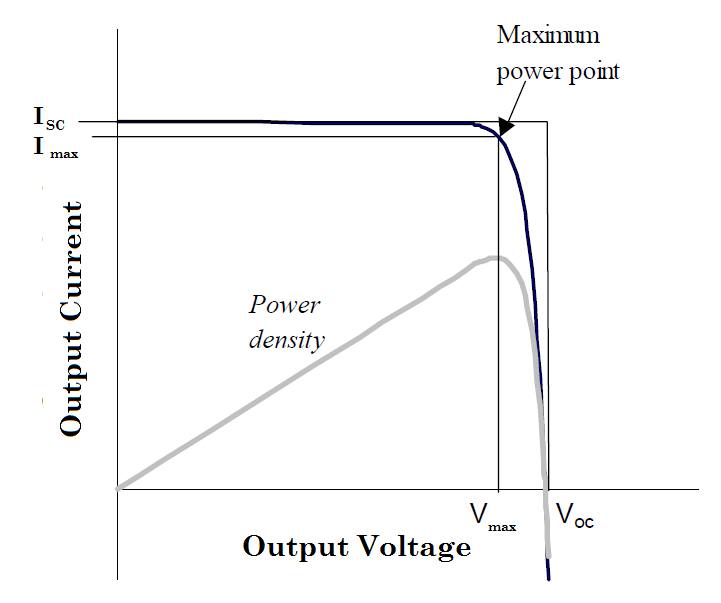
\includegraphics[width = 3.5in]{IV_curve_solar.PNG}
\caption{Output Voltage Vs. Current of a Solar Cell}
\label{Output Voltage Vs. Current of a Solar Cell}
\end{figure}

Drawing maximum power from the solar unit requires a specific DC load which optimizes the product of photocurrent and output terminal voltage to produce the largest possible value. This sourcing configuration is known as the maximum power point that a solar inverter will ideally operate at by varying its impedance. The I-V curve indicates best performance for energy generation when it closely matches a square since this maximizes the power density of the solar cell. Deviations from this optimal shape occur due to the parasitic elements in the engineering model. Output current can be undesirably leeched through the parasitic shunt resistance $R_{sh}$ which is due to current leaks in the semiconductors. The output current is also hindered by the series resistance $R_{s}$ which is present due to contact resistances. Larger $R_{sh}$ and smaller $R_{s}$ values indicate higher quality solar cells. Increased temperatures will also negatively effects the cells by decreasing the maximum possible output voltages.

Solar cells each typically produce under 1V, so multiple cells are be connected in series to create a panel with a useful voltage range. The forward diode in the cell's circuit model has the possibility of drawing current from neighboring cells when they are collected in parallel. Reversed blocking diodes are placed within the panel circuit to mitigate this as the individual cell outputs vary. The complete solar panel features many submodules of solar cells connected to a DC bus network which are then interface with polarized output leads.

\section{The Hybrid Inverter Team Development Board}
The Hybrid Inverter Team's development board aims to be a higher power replacement for TI's Solar Explorer development board with several key changes. Several of the auxiliary modules included with the Solar Explorer that were unnecessary for our design were omitted. The omitted modules included the second microcontroller for solar panel emulation, as well as the SEPIC converter used for battery charging. With the already lofty goal of building a full switch-mode boost and inverter, we felt it would be a great deal of added complexity to build, code, and troubleshoot the SEPIC battery charger for our senior design project. The panel emulator was unnecessary since we would either be running the board from an ATX power supply, or a real solar panel.

Our PCB layout utilizes a four layer design with power and ground planes on the two middle layers. Multiple layers allow for components to be placed closer together to achieve a smaller overall form factor. Additionally, there are polygon pours on the central power layers to increase current carrying capacity and aid in the dissipation of heat. Ground plane isolation is used to separate areas with switching power signals and digital logic.

Development of the PCB layout was done with EAGLE to create the top layer as shown in Figure ~\ref{PCB top} and the bottom layer shown in Figure ~\ref{PCB bottom}. The board house Advanced Circuits was used for fabrication while components were purchased from Digi-Key. The completed circuit board is displayed in Figure ~\ref{hybrid_PCB}. 
 

\begin{figure}
\centering
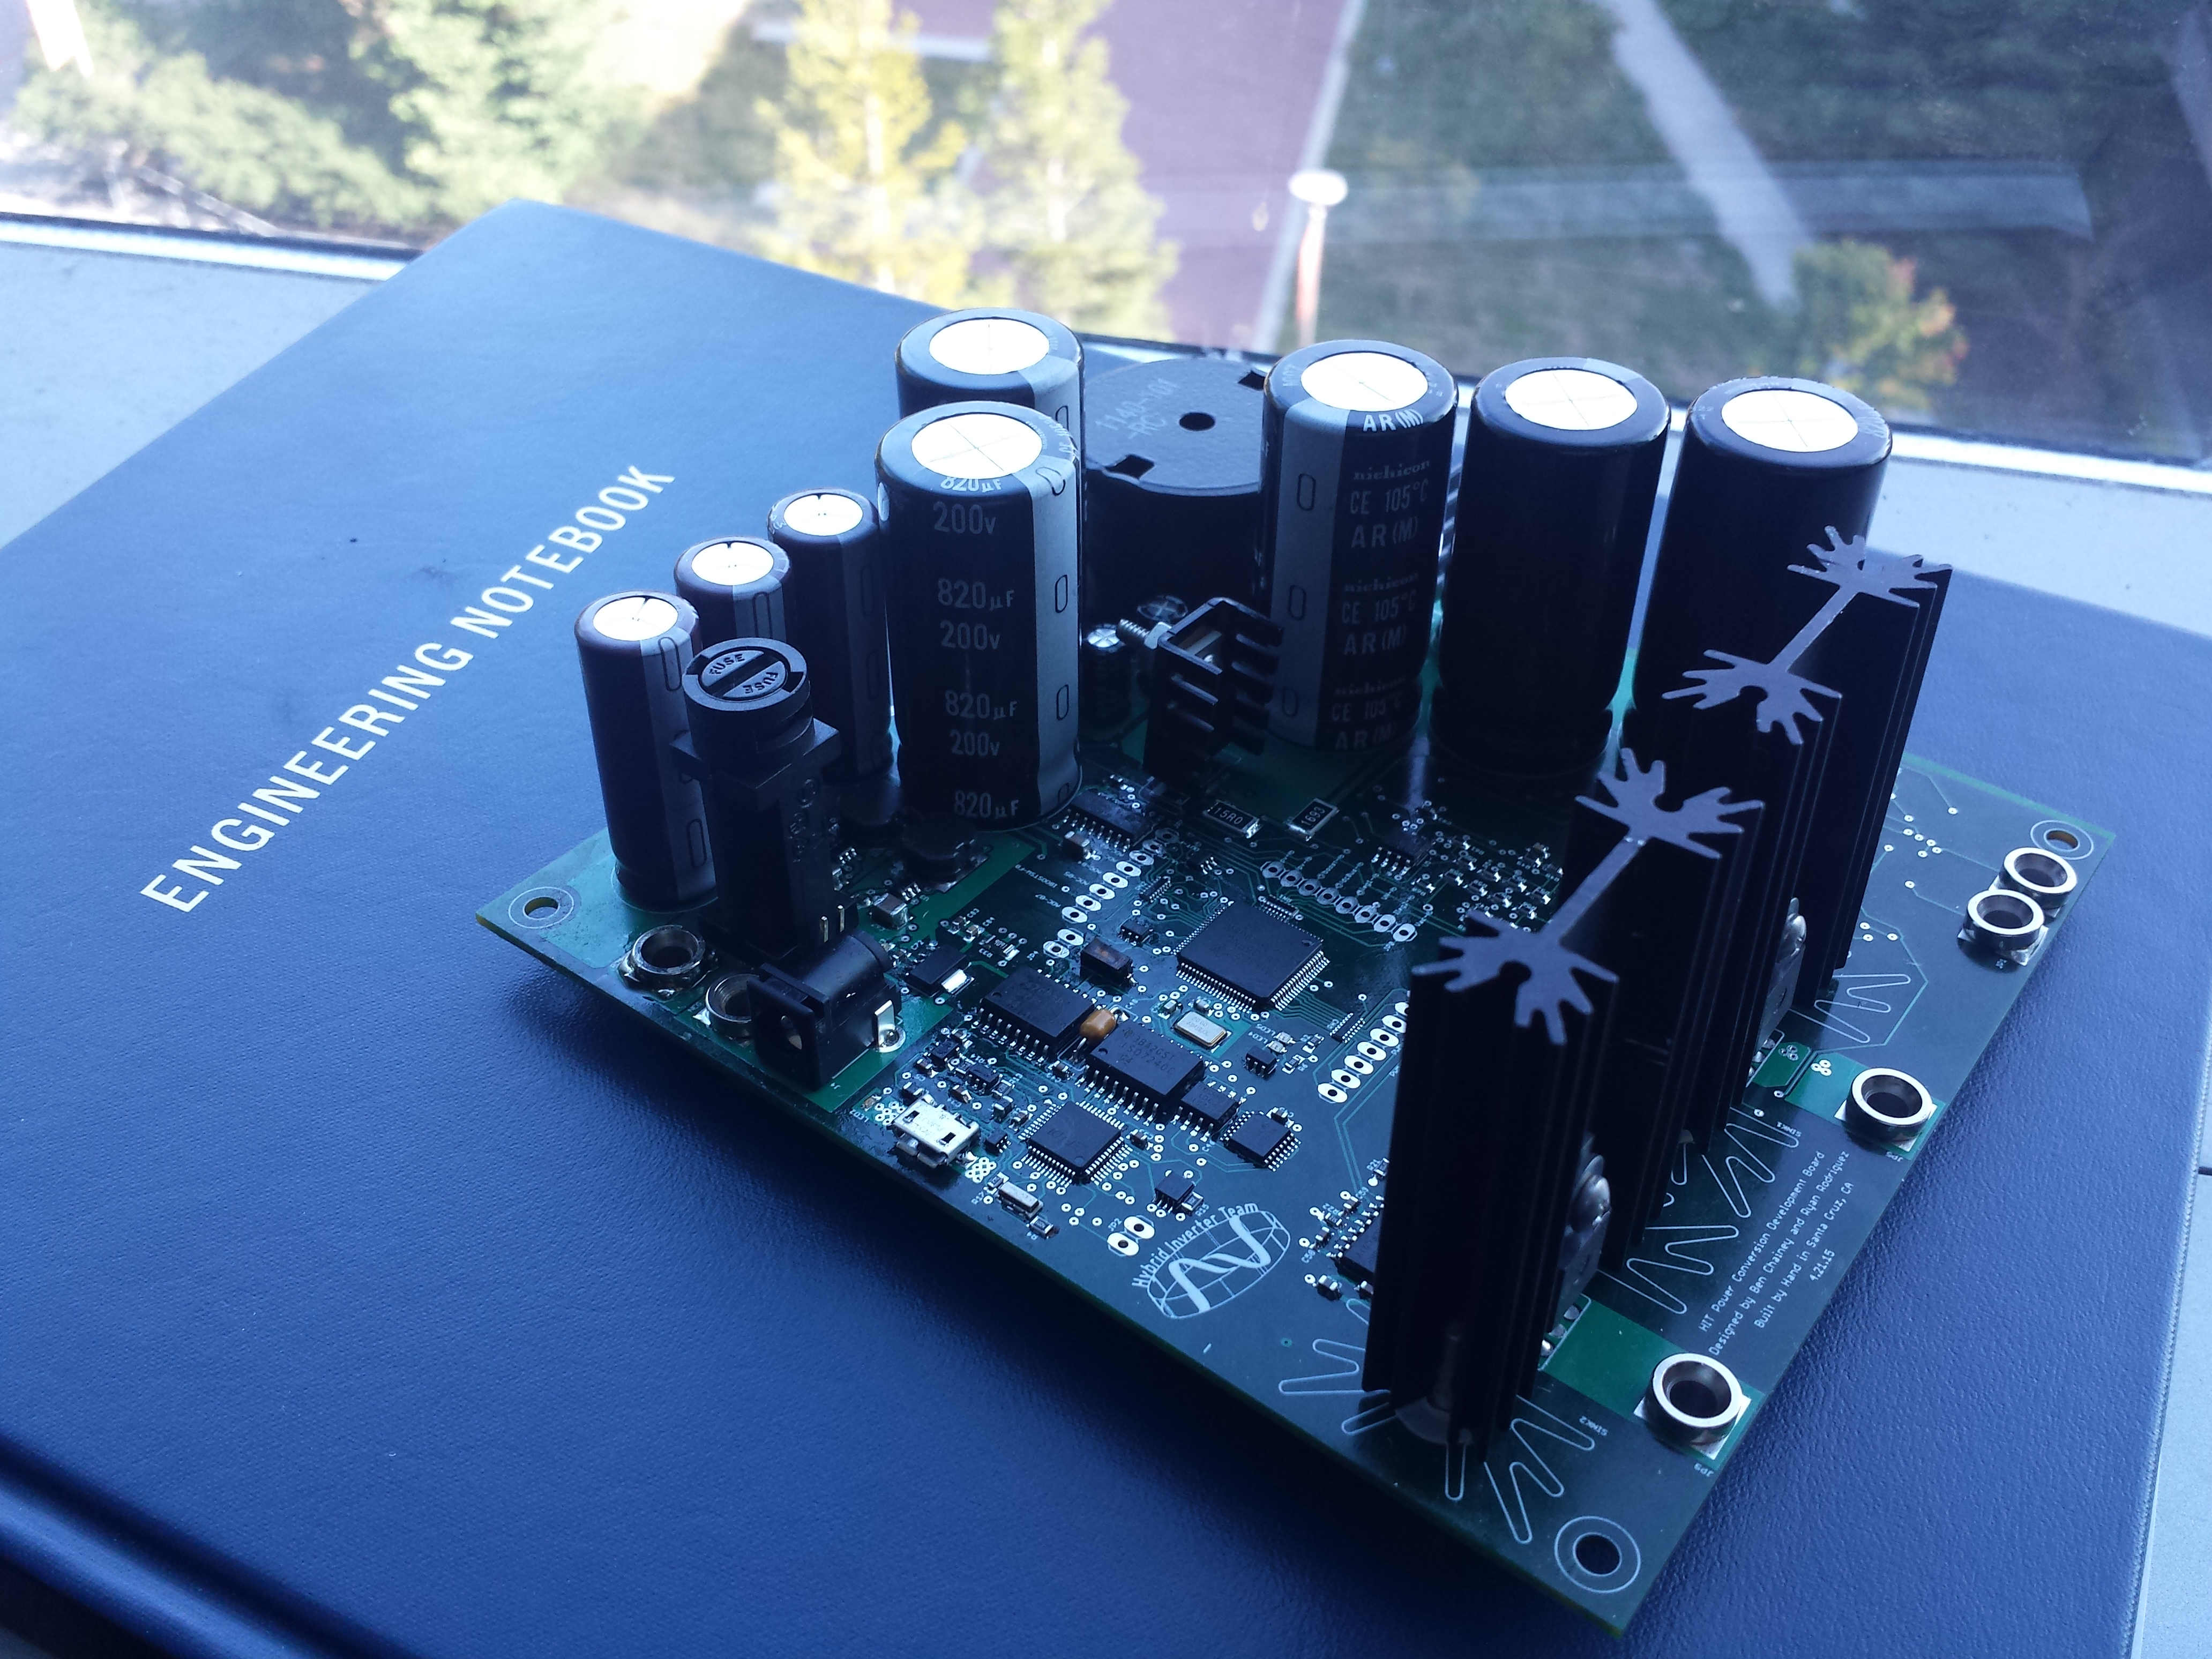
\includegraphics[width = 3.5in]{hitDevBoard}
\caption{The Hybrid Inverter Team's assembled PCB}
\label{The Hybrid Inverter Team's assembled PCB}
\end{figure}


Following the microinverter topology, the inverter sits in an enclosure mounted to the back of a solar panel. The output filter and transformer are constructed using turret board, and are also attached on the panel mounting system. For testing in outdoor sunlight environments, a wooden stand for the solar panel and inverter system is used as shown in Figure~\ref{solar stand}.

\begin{figure}
\centering
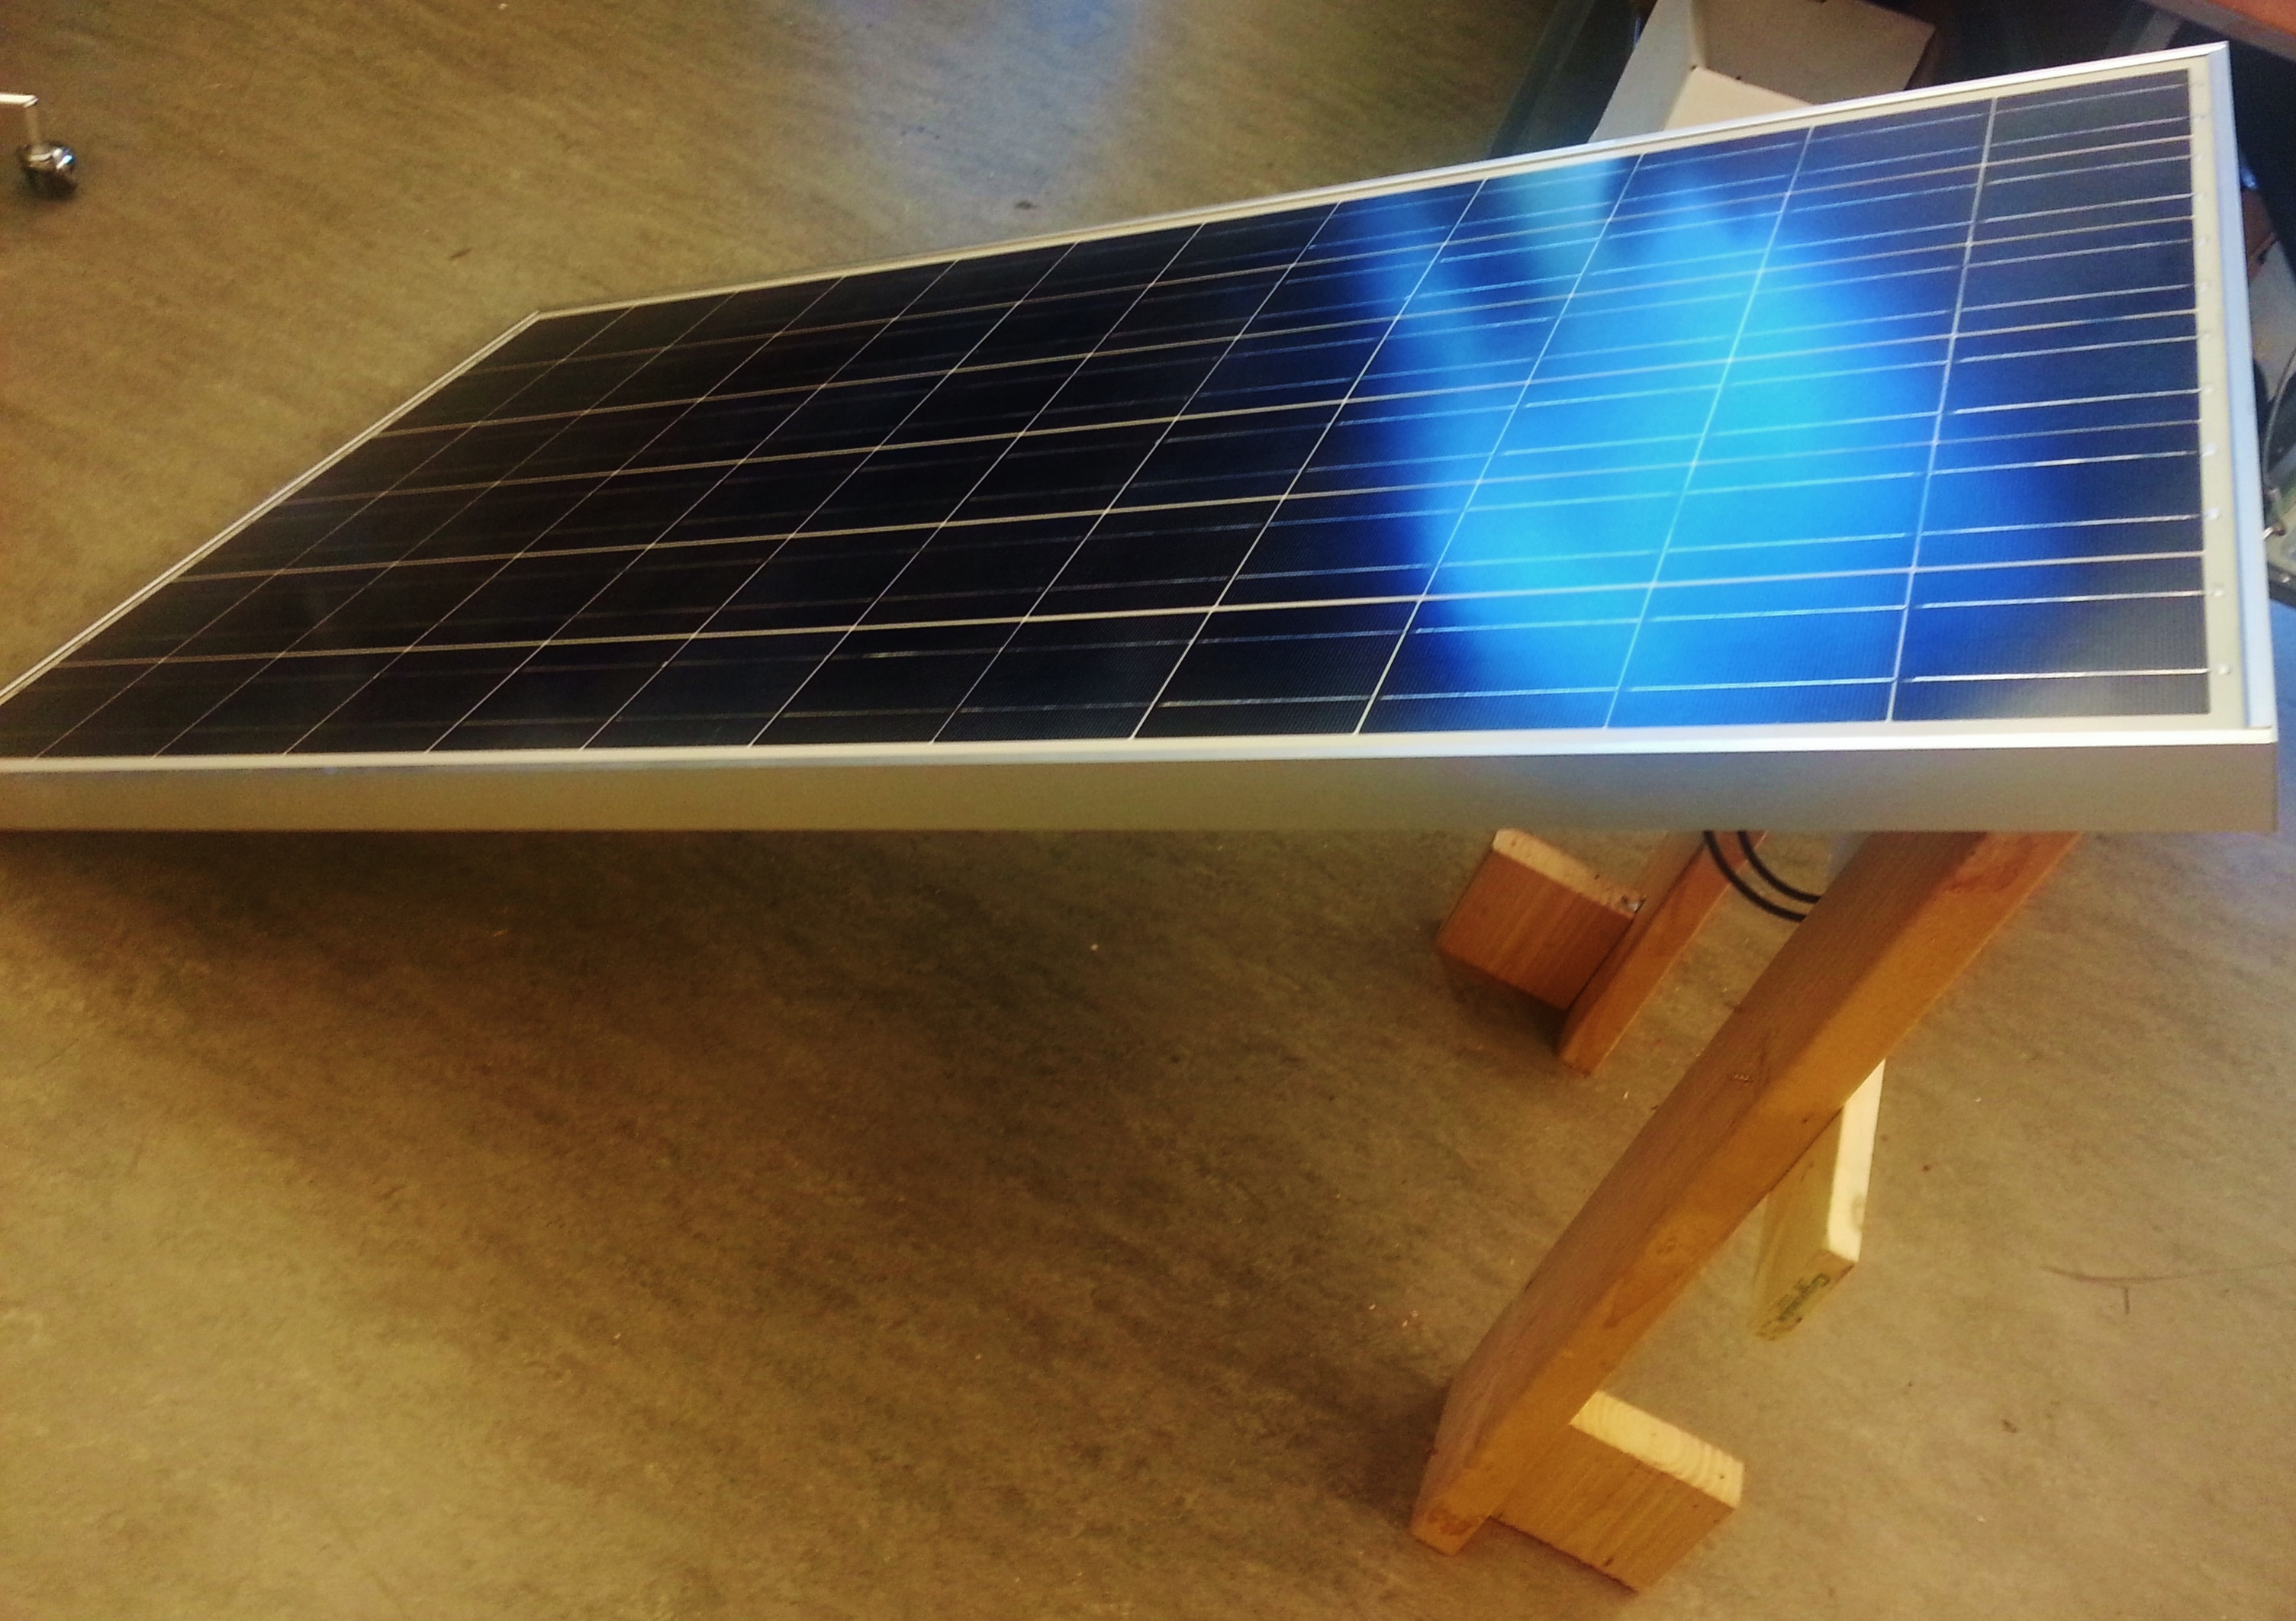
\includegraphics[width = 3.5in]{solar_stand.jpg}
\caption{Solar Panel Stand}
\label{solar stand}
\end{figure}

\subsection{Revision Two of the Hybrid Inverter Team Board}
Revision one was found to have a few weak links in the signal chain, namely an undersized trace from the source of the boost FET to the shunt resistor in the path to ground, and a microcontroller layout that was too ambitious given the debugging timeframe. We opted to replace the microcontroller layout with a 100-dimm slot capable of holding a TI ISO-control card. This alleviated the possibility of a small error in the micro layout derailing our progress, and also had the added benefit of shriking our board layout slightly. The rearrangement of components necessitated a re-pouring of some power planes to accomodate capacitors that were placed closer to the H-bridge. The new layout facillitated cutouts in the ground plane that vectored high current injections to the ground plane around both the microcontroller and the sense circuitry. Because banana plugs are relatively expensive and bulky, we ommited a pair dedicated to retrieving feedback signals from the offboard filter with pin headers as these signals are not particularly high current. 
